\documentclass[oneside, 10pt]{article}

\usepackage{amsmath}
\usepackage{amsfonts}
%\usepackage{algorithm}
%\usepackage{algorithmic}
\usepackage{multirow}
\usepackage{colortbl}
\usepackage{color}
\usepackage[table]{xcolor}
\usepackage{epigraph}
%\usepackage{subfigure}
\usepackage{caption}
\usepackage{subcaption}
\usepackage{tabularx}
\usepackage{float}
\usepackage{longtable}
\usepackage[pdftex]{graphicx}
\usepackage{pdfpages}
\usepackage{tabularx}
\usepackage{pdflscape}
\usepackage[acronym,toc]{glossaries}
\usepackage[margin=1.2in]{geometry}
\usepackage{titling}

\usepackage[style=ieee,backend=biber]{biblatex}
\addbibresource{report.bib}


\providecommand{\tightlist}{%
	\setlength{\itemsep}{0pt}\setlength{\parskip}{0pt}}
\setcounter{secnumdepth}{0}

\PassOptionsToPackage{hyphens}{url} % url is loaded by hyperref
\usepackage[unicode=true]{hyperref}

\setlength{\parindent}{0pt}
\setlength{\parskip}{6pt plus 2pt minus 1pt}


\pretitle{%
	\begin{center}
		\huge
		
\includegraphics[width=6cm,height=2cm]{images/reading_logo.png}\\[\bigskipamount]
	
	}
\posttitle{
	
	\large
	School of Mathematical, Physical and Computational Sciences
	
	Indivdual Project - CS3IP16
\end{center}}


\title{Opinion Mining and Social Media Sentiment Analysis in the Prediction of Cryptocurrency Prices}
\date{Submission date: Place Holder}
\author{Student: Andrew Sotheran
	\\Student Number: fr005432
	\\Supervisor: Kenneth Boness
	\\Word Count: Place Holder}

\begin{document}
	
	\maketitle
	
	\vspace*{\fill}
	\begin{center}
		\section{Abstract}\label{abstract}
	\end{center}
		The volatility of the stock markets is an aspect that is both hard to predict and to mitigate particularly when relating to the cryptocurrency market. Commodities such as cryptocurrencies are profoundly volatile and have attracted investors in an attempt to make quick profits on the market. These financial commodities are subject to the whim of public confidence and platforms such as Twitter and Facebook are most notably utilised to express opinions. Extrapolating sentiment from such platforms has been used to gain insight into topics across industries, thus applying it to crypto-market analysis could serve to show a relationship between public opinion and market change. 
		
		This project looks into public perception of the cryptomarket, by analysing Bitcoin-related tweets per hour for sentiment changes that could indicate a correlation to market fluctuations in the near future. This is achieved by training a recurrent neural network on the severity changes of historical sentiment and price over the past year every hour. The predictions are then shifted forward in time by 1 hour to indicate the corresponding Bitcoin price interval.

	
	\newpage
	\begin{center}
		\section{Acknowledgements}\label{acknowledgements}
		I would like to express my gratitude to Dr. Kenneth Boness for his continued support and guidance throughout this project.  
		
		Secondly, I want to express gratitude to PhD. Jason Brownlee, of \href{machinelearningmastery.com}{Machine Learning Mastery} for having clear and thorough explanations of machine learning concepts and metrics.
		
		I would also like to thank my family for their support during the development of this project.
		
	\end{center}
	
	\newpage
	\begin{center}
		\section{Glossary}\label{glossary}
	\end{center}
	Bull(ish)/Bear(ish) Markets - Relates to a trend of the market price increasing and decreasing respectively
	
	Highs/Lows - The highest and lowest trading price of a giving period
	
	Fiat Currency - A currency without intrinsic value that has been established as money
	
	BTC - Bitcoin's stock symbol
	
	Twitter - Online social media platform, which allows users to post information or express opinions through messages called "Tweets"
	
	Tweets - The name given for messages posted on the Twitter platform, which are restricted to 280 characters.
	
	Hashtag - Is a keyword or phrase used to describe a topic and allows the tweets to be categorised.
	
	Fomo (Fear of Missing Out) - Is used to describe buying behaviour when stocks are moving suddenly and more buyers appear to enter all of a sudden.
	
	Shorting - Or short sale, is the sale of an asset that the investor buys shares and immediately sells them, hoping to make a profit from buying later at a lower price.
	
	Doubling Down - Is to take further risk on a stock by doubling effort/investment in a hope and attempt to raise the price
	
	RNN - Recurrent Neural Network
	
	LSTM - Long-Short Term Memory Neural Network
	
	\newpage
	
	\begin{center}
		\tableofcontents
	\end{center}
	
	\newpage
	\begin{center}
		\section{Introduction}\label{introduction}
	\end{center}
	The premise of this project is to investigate into whether the sentiment in social media has a correlation to the prices of cryptocurrencies and how this could be used to predict future changes in the price. 
	
	The chosen cryptocurrency that will be focused in this project will be the currency that has the most community and backing and has been known to lead other fiat currencies, Bitcoin (BTC). Bitcoin is seen as one, if not the first cryptocurrency to bring a wider following to the peer-to-peer token transaction scene since 2009. Although it was not the first token to utilise blockchain technology, it allowed investors to openly trade a public cryptocurrency which provided pseudonymous means of transferring funds through the internet. Thus it has been around longer than most of the other fiat currencies and is the most popular crypto-token due to it's larger community base.
	
	Most financial commodities are subject to the whim of public confidence and are the core of it's base value. A platform that is frequently used for the public to convey their opinions on a commodity is that of Twitter which provides arguably biased information and opinions. Whether the opinions present a basis in facts or not, they are usually taken at face value and can influence the public opinion of given topics. As Bitcoin has been around since 2009 the opinions and information on the commodity are prevalent through the platform. 
	In the paper \textit{Sentiment Analysis of Twitter Data for Predicting Stock Market Movements} by \textit{Majhi et al.} \cite{1} 2.5 million tweets on Microsoft were extracted from Twitter, sentiment analysis and logistical regression performed on the data yielded 69.01\% accuracy for a 3-day period on the increase/decrease in stock price. These results showed a "\textit{good correlation between stock market movements and the sentiments of public expressed in Twitter}".
	
	The background of this project is in response to the volatility of the cryptocurrency market, which can fluctuate at a moments notice and can be seen to be social media driven. The history of the price of Bitcoin and what was being discussed on the currency around it's most volatile period to-date, Nov-2017 to Feb-2018, shows a strong bullish trend which saw Bitcoin reach a \$19,500 high in mid-Dec. While social media, such as Twitter, during that period was had an extremely positive outlook on the cryptocurrency. The trend was short lived and saw the market crash only a month later, with only a couple of sell-offs, expected for the holidays rush, accompanied by negative outlooks posted on social media turned the market against itself which saw the longest bearish market in Bitcoin's history and is still trying to recover today.
	
	Due to how volatile the crypto-market can be, there is a need to either mitigate or to anticipate where the markets are heading. As the crypto-market and Bitcoin are affected by socially constructed opinions, either through Twitter, news articles or other forms of media, there is a way to perform the latter, where the prices of Bitcoin could be predicted based on the sentiment gathered from social media outlets.
	
	The aim of this project is to create a tool that gathers tweets from Twitter, obtains the overall sentiment score of the given text while gathering historical price data for the time period gathering occurs. Features are then extracted from the gathered data and used in a neural network to ascertain whether the price of the currency can be predicted from the correlation between the sentiment and price history of the data.
	
	This report will discuss the justifications for the project and the problems it will be attempting to resolve, the stakeholders that would benefit the most from this system and what this project will not attempt to accomplish. Similar tools will be critiqued and examined for their feature set and credibility in the literature review along with current sentiment analysers, algorithms, natural language processing techniques and neural networks in their respective topics and comparing their accuracy for this project purpose. 
	The solution approach will discuss the decisions and reasoning behind choosing the techniques and tools used for this project and will outline the requirements for this project.
	Implementation of the chosen techniques and tools, with the discussion of important functions of the system will formulate the implementation section of this report with an in-detail explanation of the function's use and data flow of the system.
	
	\newpage
	
	\begin{center}
		\section{Problem Articulation}\label{problem}
	\end{center}
		
		\subsection{Problem Statement}\label{statement}
		
		The key problems this project attempts to address are that of, an open-source system available to the public that aids in the analysis and prediction of BTC. The accuracy of open-source tools and technology when applied to the trading market scene and to identify whether there is a correlation between Twitter sentiment and BTC price fluctuation. While there are existing tools only a few are available to the public and only provide basic functionality, while others are kept in-house of major corporations who invest into this problem domain.
		
		The other issue presented here is that assuming perfect accuracy can be achieved is naive. As this project will only be using existing tools and technologies thus, there are limitations to accuracy that can be obtained. One of that being the suitability of the tools, there are no open-source sentiment analysers for stock market prediction, thus finding a specifically trained analyser for the chosen domain in highly unlikely. In relation, finding the most suitable machine learning or neural network is equally important as this will determine the accuracy of the predictions. Due to being a regression problem, machine learning techniques and neural networks that focus around this and forecasting should be considered.
		
		The accuracy and suitability of various machine learning methods and neural networks are a known issue in their respective domains, this investigation should be carried out to determine their suitability for their needed use in this project and should be detailed in the literature review.
		
		This project will focus on the investigation of these technologies and tools to justify whether it is feasible to predict the price of BTC based on historical price and the sentiment gathered from Twitter. Limitations of the system and it's accuracy in predictions should be investigated and discussed to determine the implemented solution is the more suitable compared to other methods.  
		
		\subsection{Stakeholders}\label{stakeholders}
		The main stakeholders of this system would be those looking to invest in the cryptocurrency markets, in this projects regard, specifically into Bitcoin. 
		
		\begin{itemize}
			\item Public Investors - These are investors from the general public. These investors can decide to either actively or passively invest in the markets but are essential for the general use of a given cryptocurrency. This type of investor would benefit the most from an open-source system such as this, as it will aim to provide a basis for decisions for buying or selling Bitcoin. Additionally, due to the lack of any open-source tools available, these stakeholders could be seen as being left in the dark when it comes to predicting the direction of Bitcoin where Businesses and Enterprises will have a one up, due to having an internal system for predictions.
			\item Speculators - These stakeholders can be both public and business, who aim for the chance of the possibility fast. They actively invest at points where a market is an impending rise in price and tend to sell after a market makes them a reasonable amount of money before it possibly drops. These stakeholders would benefit from such a system as it will provide a means to identify and predict short term gains in the Bitcoin market, and if taken into decisions could make a profit.
			\item Business Investors: These will be investors of a business who would be investing on the behalf of a company. A system such as that this project will provide may benefit such a stakeholder, but the information would be used as a collective with others to justify the investment. Additionally, this system may not benefit this stakeholder as the company they are investing for may have an equivalent or better system.
			\item Prospect Investors: These are new investors to the cryptomarket scene who are looking to get into the market and are generally looking for initial information of the market movement. This system will benefit such a stakeholder in their initial decisions in market investment, but not as much as a generally more active investor. This is due to the extent to which a new investor invests compared to a establish active investor.
			
			\item Developer - Andrew Sotheran: The developer responsible for this project by developing a solution that satisfies the problem and	objective defined in the \textit{Technical Specification}. As the sole developer of this project it should be ensured that the system is developed on time and the project runs smoothly.
			\item Project Supervisor - Kenneth Boness: Is the projects supervisor whom will oversee the development through weekly project meetings. Weekly feedback will be given on the progress and direction of development, and will offer advice to ensure the quality of the solution.
		\end{itemize}
		
		\subsection{Project Motivation}
		The motivation behind the project stems from a range of points, from personal and public issues with the volatility if the crypto-market, and how losses specifically could be mitigated. The personal motivations behind the conceptualisation of this began two years ago during the crash of late 2017-2018, which saw new investors blindly jump into the trend that was buying cryptocurrencies. During this period of November to December 2017 saw Bitcoin's price reach \$20,000 from \$5,000, new public investors jumped on the chance to buy into the trend of possibly making quick profits and the fear of missing out (FOMO). In late December, a few holiday sell-offs occurred from business and big investors, this coupled with a few negative outlooks posted on social media by news outlets caused the market to implode causing investors to panic sell one after the other and posting negativity on social, thus causing more decline in the market. As a result, this caused personal monetary loss and distress as being a long-term investor.
		
		Another motivation is that at the time of writing, there are no pubically available systems that combine sentiment analysis with historical price to forecast the price of Bitcoin or any other cryptocurrency. There are papers and a few code repositories that implement a similar concepts \cite{2} - \textit{Use of a Multi-layer Perceptron network for moving averages in Bitcoin price}, \cite{3} - \textit{Predicting Bitcoin price fluctuation with Twitter sentiment analysis}, \cite{4} - \textit{Predict Tomorrows Bitcoin (BTC) Price with Recurrent Neural Networks} but are not operational. System such as \cite{1} hosted on Coingecko, a popular cryptocurrency track site, provides a tool for basic sentiment analysis but doesn't give an evaluated indication of the direction of the market as a prediction. This leaves the public to the whim of volatility of the market without a means to know what the next, say an hour, could entail to possibly reduce losses if the market drops. Such system are usually kept in-house of major corporations whom invest significant time into tackling such a problem. Additionly, this could be seen as a positive for major investors, as such a system could cause panic selling if public investors soley trusted such a system.
			
		\newpage
		\subsection{Technical Specification}
		This project will need to follow a specification to ensure that the quality and the problem statement is met. This section will outline what this project should include, what it will not consist of and will guide the development of this project.
		\newline
		
		\textbf{General}:
		\begin{itemize}
			\item To investigate into the use of lexicon-dictionary based sentiment analyser approach in for sentiment analysis and it's customisability for a given topic domain
			\item To create a system that can predict the next hour of Bitcoin’s price when given the price and sentiment for the past hour
			\item To investigate into natural language data pre-processing techniques and how these could be used to filter out unwanted data
			\item To investigate into the use of a neural network, specifically an LSTM for forecasting price data
			\item Ultimatly, to investigate into how the use of sentiment effects the prediction of price for the next hour
			\newline
		\end{itemize}
		
	
		\textbf{Natural Language pre-processing (Spam and language detection filtering)}
		\begin{itemize}
			\item To produce a system that processes the historical and live tweets, removing unwanted characters, removing urls and punctuation.
			\item To produce a system for spam filter using probability likelihood for processed tweets. A naive Bayes approach may be suitable for this given task
			\item To produce a language detection and filtering system that removes all tweets that are not of the English language or containing non-basic-latin characters
			\item To provide a means for stemming, tokenisation and stopword removal to aid in data pre-processing for language detection and spam filtering
			\newline
		\end{itemize}
		
		\textbf{Neural Network}
		\begin{itemize}
			\item To produce a neural network which trains on collected, historical and live data, to forecast the future price of Bitcoin, based on price and sentiement
			\item To produce a neural netowork which accomplished the same as the other above, but with out use of sentiment
			\item To produce metrics to justify accuracy of the model
			\item To produce data files containing, the current time of predictions alongside current hour price and sentiment. This should also include a suggested action based on a threshold for the price difference between hours. 
			\item To produce JSON files containing the true and predicted price values of every hour for trained data, and another for current reoccuring predictions.
			\newline
		\end{itemize}
		
		\textbf{Interface}
		\begin{itemize}
			\item To produce a basic interface which displays the predicted values alongside true price values with a time interval step of an hour. This can be displayed as both a table consisting of: 
			\subitem Date of prediction, predicted price of next hour, current hour price and sentiment, and a suggested action based on a threshold for the price difference between hours.
			\subitem To produce charts displaying the true and predicted price values for every hour, from both start of new predictions made, and from training predictions
			\item To display a table of performance metrics of the trained model
			\newline
		\end{itemize}
	
		\textbf{Server}
		\begin{itemize}
			\item This system, both prediction system and interface, should be deployed to a server due to the need to be constantly running
		\end{itemize}
		
		\subsection{Project Constraints}\label{constraints}
		
		This project will not attempt to justify the accuracy of the chosen algorithm or tools over other algorithms. It will be discussed in the solution approach the justifications made on why the chosen algorithm and tools have been used for this project over the others, but accuracy will not be directly compared.
		
		This project will only be coded to predict an hour ahead as the model will be trained on an hourly basis as the data is gathered per hour. Predictions for further in the future can be modelled but will be seen as a future improvement to the system.
		
		The detail of a interface may be subject of change through this project due to time contraints and the focus being the investigation of the impact social media has on market predictions.
		
	
	\newpage
	
	\begin{center}
		\section{Literature Review}\label{literature}
	\end{center}
		\subsection{Existing Tools}
		An aspect that this project will be attempting to address is that, at the time of writing, there are a limited amount of systems available to the public that either provide sentiment analysis or predictions of the crypto-market. Additionally, none known that combine both sentiment and price analysis to make said predictions on the direction of the market.
		
		Such tools are usually provided by exchanges which correspond the amount of positive and negative sentiments with a suggestion to buy and sell. These tools, however, are vague in their suggestions as they don't provide any further analysis on when the best time would be to conduct an action on the market, and simply display the number of tweets per sentiment level. A well-known cryptocurrency tracking site,\href{https://www.coingecko.com}{Coingecko} provides a basic sentiment analysis tool for their top 30 ranking cryptocurrencies tracked on the site. This tool shows the sentiment analysis of tweets from Twitter every hour for a given cryptocurrency. This is displayed as a simple pill on the page showing the ratios of positive, neutral and negative tweets. \textit{See Appendix C for visual representation}
			
		\subsection{Related research}
		
		There has been a plentiful amount of research conducted in this problem domain. Numerous theses globally have been published in recent years on the topic of cryptocurrency market predictions and analysis, and even more, research conducted on general stock markets further back. 
		
		The thesis written by \textit{Evita Stenqvist and Jacob Lonno} of the \textit{KTH Royal Institute of Technology} \cite{3} investigates the use of sentiment expressed through micro-blogging such as Twitter can have on the price fluctuations of Bitcoin. Its primary focus was creating an analyser for the sentiment of tweets more accurately \textit{"by not only taking into account negation, but also valence, common slang and smileys"}, than that of former researchers that \textit{"mused that accounting for negations in text may be a step in the direction of more accurate predictions."}. This would be built upon the lexicon-based sentiment analyser VADER to ascertain the overall sentiment scores were grouped into time-series for each interval from 5 minutes to 4 hours, along with the interval prices for Bitcoin. The model chosen was a naive binary classified vectors of predictions for a certain threshold to \textit{"ultimately compare the predictions to actual historical price data"}. The results of this research suggest that a binary classification model of varying threshold over time-shifts in time-series data was "lackluster", seeing the number of predictions decreasing rapidly as the threshold changed. This research is a good basis of starting research upon, as it suggests tools such as VADER for sentiment analysis and that the use of a machine learning algorithm would be a next step in the project that would yield better more accurate results.
		
		Another thesis written by \textit{Pagolu, Venkata Sasank and Reddy Kamal Nayan, Panda Ganapati and Majhi, Babita} \cite{1} on "Sentiment Analysis of Twitter Data for Predicting Stock Market Movements" 2.5 million tweets on Microsoft were extracted from Twitter, sentiment analysis and logistical regression performed on the data yielded 69.01\% accuracy for a 3-day period on the increase/decrease in stock price. These results showed a "\textit{good correlation between stock market movements and the sentiments of the public expressed in Twitter}". Using various natural language pre-processing tweets for feature extraction such as N-gram representation the sentiment from tweets were extrapolated. Both Word2vec and a random forest classifier were compared for accuracy, Word2vec being chosen over the machine learning model. Word2vec, being a group of related shallow two-layer neural network models to produce word embeddings.
		
		A topic that reoccurs in various papers and theses is that of the use and focus of regression techniques and machine learning methods. Few implement a fully fledged neural network, the above paper attempts to use a simple network to achieve predictions of classification of sentiment for stock market movement then correlated this with historical data of prices. An article posted on "Code Project" by Intel Corporation \cite{5} compares the accuracy of three machine learning algorithms; Random Forest, Logistic Regression and Multi-Layer Perceptron (MLP) classifiers on predicting the price fluctuations of Bitcoin with embedded price indices. Results showing \textit{"that using the MLP classifier (a.k.a. neural networks) showed better results than logistic regression and random forest trained models"}. This assumption can be backed up by the results from a thesis posted on IEEE \cite{6} which compares a Bayesian optimised recurrent neural network and a Long Short Term Memory (LSTM) network. Showing the LSTM model achieving \textit{"the highest classification accuracy of 52\% and a RMSE of 8\%"}. With an interest in neural networks personally and with little papers utilising them for this purpose a neural network will thus be implemented, and the accuracy of one's predictions with use of sentiment analysis data analysed and discussed.
			
		\subsection{Data Collection}\label{tweet_collection}
			
			\subsubsection{Twitter and Twitter API}
			Twitter is a micro-blogging platform that was launched in 2006 and provides it's users the ability to publish short messages of 140 characters. The messages published could be of any form, from news snippets, advertisement, or the prevalent publication of opinions which allowed a platform of extensive diversity and knowledge wealth. As of the time of writing, the message character limit was increased to 280 characters, the platform has over 300 million monthly active users and around 1 million tweets are published per day. Due to the length restriction and the primary use of the platform to express opinions Twitter is seen as a gold mine for opinion mining.
			
			The Twitter API has an extensive range of endpoints	that provide access from streaming tweets for a given hashtag, obtaining historical tweets for a given time-period and hashtag, posting tweets on a users account and to change settings on a user account with authentication. The exhaustive range of features provided by these endpoints makes data collection from Twitter straight forward as one can target a specific endpoint for the required data. Due to Twitter being the target for opinion mining within this project the Twitter API will ultimately need to be utilised. This can either be used for the gathering of historical tweets or streaming current tweets for the \#Bitcoin hashtag.
			
			There are, however, limitations and rate limits imposed on users of the API. Twitter employs a tiering system for the API - Standard, Premium and Enterprise tiers, each of which provides different amounts of access for data collection. If the API were used to capture historical data for a span of 3 months, each tier is allowed to obtain varying amounts of data for different durations; \cite{7}
			
			\begin{itemize}
				\item A Standard user would be able to capture 100 recent tweets for the past 7 days
				\item A Premium user would be allowed to capture up to 500 tweets per request for a 30-day span and will have access to a full-archive search to query up to 100 tweets per request for a given time period, with a 50 request limit per month
				\item An Enterprise user would be able to capture up to 500 tweets per unlimited requests for a 30-day span and will be able to query the full-archive of tweets for a given hashtag up to 2000 tweets per unlimited amount of requests for a given time period
			\end{itemize}
		
			Each tier has individual costs while the standard user negating this as a basic tier. Due to only being elegable for the Premium tier for educational purposes, historical data gathering will be limited to 100 tweets per request with a limitation of 50 requests per month. Furthermore streaming tweets is an Enterprise feature which rules out the the Twitter API for use of streaming current real-time data \cite{8}.
		
			\subsubsection{Tweepy Python Package}
			Tweepy is a python package for accessing the Twitter API. It fundamentally accomplishes the same means if one to conduct a GET request to the Twitter API, except it simplifies this into a simple to use API that is easier to implement and automate in python \cite{9}. Consequently, it builds upon the existing Twitter API to provide features such as automated streaming of provided hashtags to the API. It realises this by initialising a listener instance for a provided set of API credentials, handling authentication, connections, creating and destroying sessions. Due to Twitter's streaming API being only available to Enterprise users \cite{7}, using Tweepy to stream data for a given hashtag will provide the real-time data needed.
			
		
		\subsection{Sentiment Analysis}\label{sentiment}
		In short, sentiment analysis is the process and discovery of computationally identifying and categorising the underlining opinions and subjectivity expressed in written language. This process determines the writer's attitude towards a particular topic as either being positive, neutral or negative in terms of opinion, known as polarity classification. 		
			
			\subsubsection{Natural Language Processing}\label{algorithms}
			Polarity classification is the focus of sentiment analysis and is a well-known problem in natural language processing that has had significant attention by researchers in recent years \cite{1}\cite{3}\cite{6}\cite{10}. Traditional approaches to this have usually been classified to dictionary-based approaches that use a pre-constructed sentiment lexicons such as VADER or usually confined to machine learning approaches. The later requires an extensive amount of natural language pre-processing to extrapolate vectors and features from given text, this is then fed into a machine learning classifier which attempts to categorise words to a level of sentiment polarity. Natural language pre-processing techniques that would be required for this approach would consist of;
			
			\begin{itemize}
				\item Tokenisation: The act of splitting a stream of text into smaller units of typographical tokens which isolate unneeded punctuation.
				\item Removal of domain specific expressions that are not part of general purpose English tokenisers - a particular problem with the nature of the language used in tweets, with @-mentions and \#-hashtags
				\item Stopword removal: Are commonly used words (such as "the","in","a") that provide no meaning to the sentiment of a given text
				\item Stemming: Is used to replace words with common suffixes and prefixes, as in "go" and "goes" fundamentally convey the same meaning. A stemmer will replace such words with their reduced counterparts
				\item Term Probability Identification and Feature Extraction: This is a process that involves identifying the most frequently used words in a given text, by using a probability type approach on a pre-defined dataset which classifies a range of texts as with overall negative or positive a machine learning algorithm is trained to classify these accordingly.
			\end{itemize}
			
			The former, seen and has been proven to provide higher accuracy than traditional machine learning approaches \cite{11}, and need little pre-proeccesing conducted on the data as words have a pre-defined sentiment classification in a provided lexicon. Although these lexicons can be complex to create, they generally require little resources to use and add to.
			
			\subsubsection{Valence Aware Dictionary and sEntiment Reasoning}\label{Vader}
				VADER is a combined lexicon and rule-based sentiment analysis tool that is specifically attuned to sentiments expressed in social media, and works well on texts from other domains. It is capable of detecting the polarity of a given text - positivity, neurality, and negativity \cite{12}. VADER uses a human-centric approach to sentiment analysis, combining qualitative analysis and empirical validation by using human raters to rate level of sentiment for words in it’s lexicon. Vader also has emoticon support which maps these colloquailisms have pre-defined intensities in its lexicon, which makes VADER specifically suitable for the social media domain where the used of emoticons, utf-8 emojis and slang such as "Lol" and "Yolo" are prevalent within text. Additionally, VADER is provided as a lexicon and a python library under the MIT license, thus means that it is open-source software. This means that the lexicon can be altered and added to making it able to being tailored to specific topic domains. 
				
				VADER was constructed by examining and extracting features from three pre-existing well-established and human-validated sentiment lexicons \cite{12} - (LIWC) Linguistic Inquiry and Word Count, (ANEW) Affective Norms for English Words, and (GI) General Inquirer. This is supplemented with additional lexicon features \textit{"commonly used to express sentiment in social media text (emoticons, acronyms and slang)"} \cite{12} and uses "wisdom-of-the-crowd" approach \cite{13} to establish a point of estimations of sentiment valance for each lexical feature candidate. This was evaluated for the impact of grammatical and syntactical rules and 7,500+ lexical features, with mean valence \textit{"<> zero, and SD <= 2.5"} as a human-validated "gold-standard" sentiment lexicon. \cite{12}\textit{Section 3.1}
				
				VADER is seen as a "Gold Standard" for sentiment analysis, in the paper for VADER, \cite{12} \textit{A Parsimonious Rule-based Model for Sentiment Analysis of Social Media Text}, it was compared against 11 other \textit{"highly regarded sentiment analysis tools/techniques on a corpus of over 4.2K tweets"} for polarity classification across 4 domains. Results showing VADER, across Social media text, Amazon reviews, movie reviews and Newspaper editorials, consistently outperforming other sentiment analysis tools and techniques showing a particular trend in performing significantly higher on analysis of sentiment in tweets. \cite{12} \textit{Section 4: Results}
			
		\subsection{Neural Networks}\label{networks}
			A neural network is a set of perceptrons modelled loosely after the human brain that is designed to recognise patterns in whatever domain it is intended to be trained on. A neural network can consist of multiple machine perceptrons or clustering layers in a large mesh network and the patterns they recognise are numerical which are contained in vectors. Pre-processed data, confined and processed into pre-defined vector labels, are used to teach a neural network for a given task. While this differs from how an algorithm is coded to a particular task, neural networks cannot be programmed directly for the task. The requirement is for them to learn from the information by use of different learning strategies; \cite{14}\cite{15}
			
			\begin{center}
				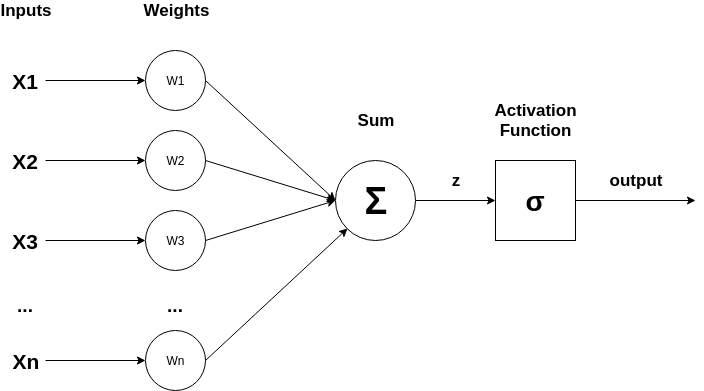
\includegraphics[width=10cm,height=6cm]{images/perceptron.png}
				\newline
				\textit{Figure 1: Basic perceptron layout}
			\end{center}
			
			\begin{itemize}
				\item Supervised learning: Simplest of the learning forms, where a dataset have been labeled which indicate the correct classified data. The input data is learned upon until the desired result of the label is reached \cite{16}
				\item Unsupervised learning: Is training the with a dataset without labels to learn from. The neural network analyses the dataset with a cost function which tells the neural network how far off target a prediction was. The neural network then adjusts input weights in attempt to increase accuracy. \cite{15}
				\item Reinforced learning: The neural network is reinforced with positive results and punished for negative results causing a network to learn over iterations. 
			\end{itemize}
		
			\subsubsection{Recurrent Neural Network (RNN)}\label{types}
			The type of neural network that is of focus for this project will be that of a Long-Short Term Memory (LSTM), however, it is important to understand how this is an extension of a Recurrent Neural Network (RNN) and how the underlying network works.
			
			Recurrent Neural Networks (RNN) are a robust and powerful type of neural network and is considered to be among the most encouraging algorithms for use of classification, due to the fact of having internal memory. RNNs are designed to recognise patterns in sequences of presented data or most suitably, time-series data, genomes, handwriting and stock market data. Although RNNs were conceptualised and invented back in the 1980s \cite{17} they've only really shown their potential in recent years, with the increase of computational power due to the level of sequencing and internal memory store to retrain.
			Due to this 'internal' memory loop, RNNs are able to remember data and adjust neurons based on failures and alternating parameters. The way this is accomplished, knowing how a standard neural network such as a feed-forward network, should initially be understood. \cite{18}
			
			A standard, feed-forward neural network has a single data flow with an input layer, through hidden computational layers, to an output layer. Therefore any node in the network will never see the same data again. However, in an RNN data is cycled through a loop over the same node, thus two inputs into the perceptron. Decisions are influenced by previous data that it has previously learned from if any, which in turn affects output and the weights of the network. \cite{19}
			
			\begin{center}
				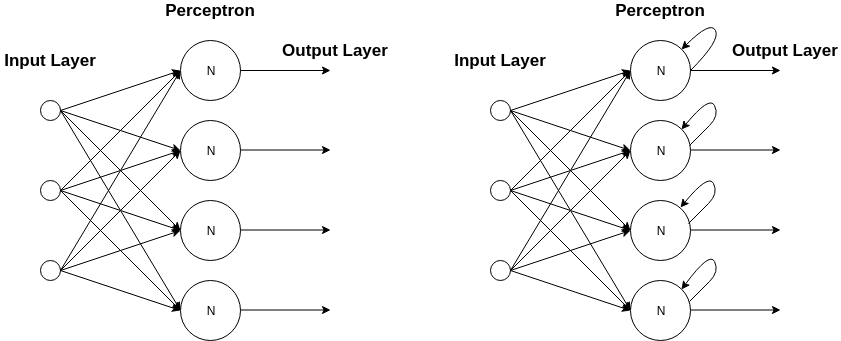
\includegraphics[width=15cm,height=6cm]{images/rnn_ffn.png}
				\newline
				\textit{Figure 2: Feed-forward network (left) vs Recurrent Neural network (right)}
			\end{center}
		
			The act of tweaking weights to alter the processing of the next iteration of data in an RNN is called backpropagation, which in short means going back through the network to find the partial derivatives of the error with respect to the weights after output has occurred. Along with gradient descent, an algorithm that adjusts the weights up or down depending on which would reduce the error. There are however a few obstacles of RNNs;
			
			\begin{itemize}
				\item Exploding Gradients: Is when gradient decsent assigns high importance to the weights. As in the algorithm assigns a ridiculously high or low value for the weights on iteration which can cause overlow and result in NaN values \cite{20}
				\item Vanishing Gradients: Is when the values of a gradient are small enough that weights cannot be altered and the model stops learning. \cite{21}
			\end{itemize}
		
			These issues are overcome by the concept of Long-Short Term Memory neural networks, coined by \textit{Sepp Hochreiter and Juergen Schmidhuber, 1997} \cite{22}. 
			
			\subsubsection{Long-Short Term Memory (LSTM)}\label{lstms}
			LSTMs are an extension of recurrent neural networks capable of learning long-term dependancies and were conceptualised by \textit{Sepp Hochreiter and Juergen Schmidhuber, 1997} \cite{22}. LSTMs were explicity designed to avoid long-term dependancy problems such as exploding and vanishing gradients. As they are an extension of RNNs they operating in almost the exact same manner, but stores the actual gradients and weights in memory which allows for LSTMs to read, write and alter the values. A way of explaining how this works is seeing the memory block as a gated cell, where 'gated' is that the cell decides whether or not to store or alter data in it's memory based input data and the importance assigned to it. In a sense it learns over time of which values and data is important.
			
			\begin{center}
				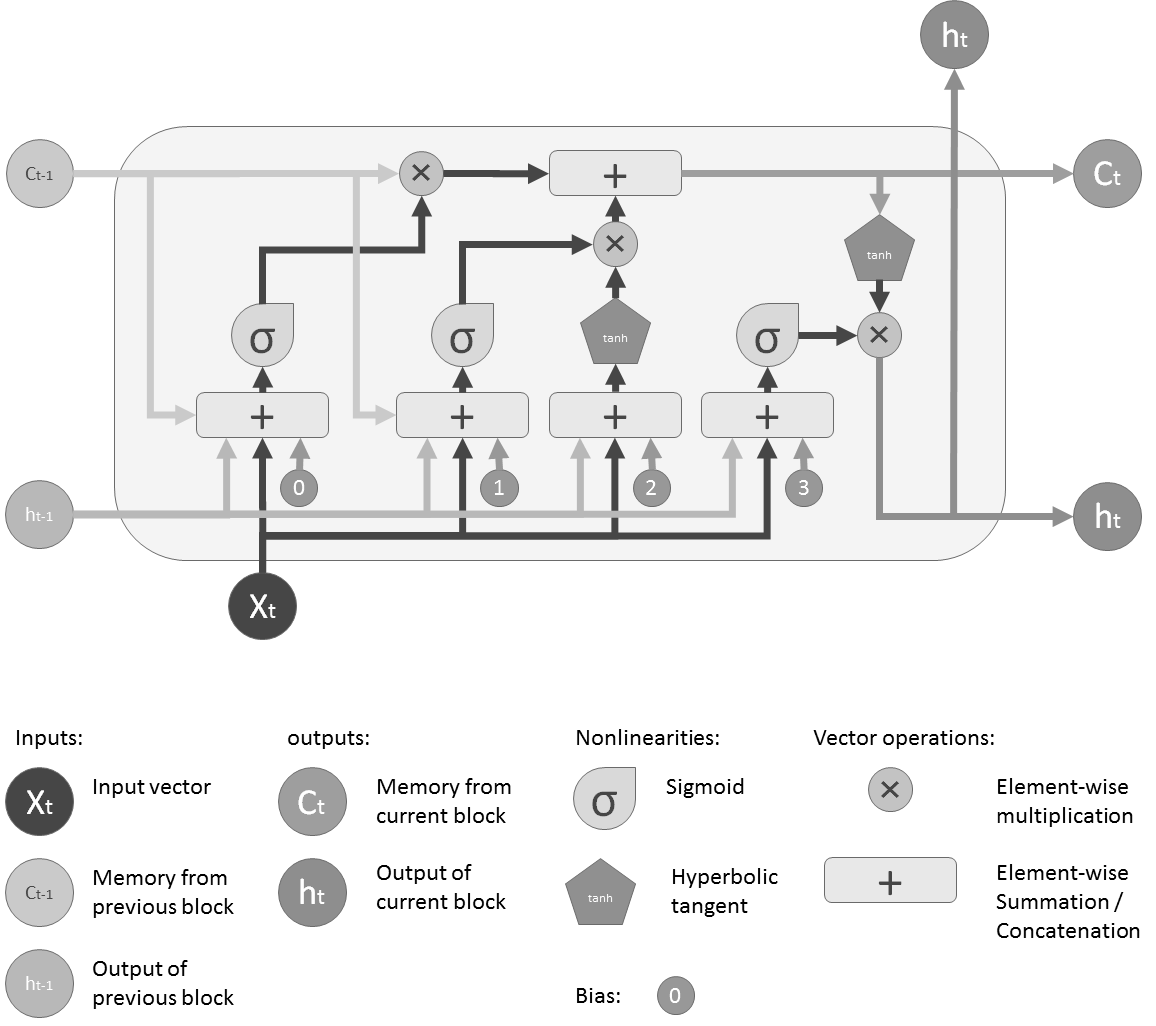
\includegraphics[width=9cm,height=7cm]{images/lstm.png}
				\newline
				\textit{Figure 3: A conceptual design of an LSTM cell bank - from Medium article by Shi Yan: Understanding LSTM and its diagrams}\cite{23}
			\end{center}
			
			The network takes in three initial inputs, input of current time step, output from the previous LSTM unit if any, and the memory of the previous unit. Outputs, $H_t$ - output of current network, and $C_t$ - the memory of the current unit. \cite{23}
			
			The various steps of the network decide what information is thrown away from the cell state, through use of a 'forget gate' which is influencted by the calculations of sigmod memory gates which influence how much of old and new memory is used $C_{t_-1}$, $H_{t-1}$
			and $X_t$, and merged together based upon importance. The section of the cell that controls the outflow memory $H_t$ and $C_t$ determines how much of the new memory should be used by the next LSTM unit. 
			\textit{For a more in-detailed explanation of exactly how the calculations are made see} \cite{22},\cite{23} and \cite{24}.
			
			As mentioned in the formost section of related work the use of an LSTM network would be optimal for the given problem domain over the use of machine learning algorithms, for time-series data. As detailed above, LSTMs are widley used for time-series data forecasting due to being able to remember previous data and weights over long sequence spans\cite{22}\cite{25}. The flexability of LSTMs such as many-to-many models, useful \textit{"to predict multiple future time steps at once given all the previous inputs"} due to use of look-back windows and control of multiple 3D input parameters.\cite{25}
			
			\subsubsection{Keras and TensorFlow}
			TensorFlow is an open-source numerical math computational library framework for dataflow differentiable programming, primarily used for machine and deep learning applications such as neural networks. TensorFlow bundles various machine learning and deep learning models and algorithms into one package for the Python language, but executes as byte code executed in C++ for performance. TensorFlow provides a range of conveniences to developers for the types of algorithms it supports such as debugging models and modifying graph operations separately instead of constructing and evaluating all at once, and compatibility to execute on CPUs or GPUs \cite{26}. However, TensorFlow's implementation and API, although provides an abstraction for development for machine and deep learning algorithms and simplifies implementation, it isn't all too friendly to programmers to use, especially new developers to the field of machine and deep learning. This is were the Keras API comes in. 
			
			Keras is a high-level built to run atop of deep learning libraries such as Tensorflow and Theanos - another deep learning library similar to Tensorflow. It is designed to further simplify the use and application of such deep learning libraries thus making implementing a neural network and similar supported algorithms friendlier to developers working in Python. It accomplishes this by being a modular API; neural layers, cost functions, optimisers, activation functions, and regularisation schemes are all standalone features of the API that can be combined to create functional or sequential models. Due to being a high-level API for more refined and easier development of deep learning libraries it does not provide these low-level operations and algorithms; Keras relies on a back-end engine such as TensorFlow and supports a wide range of others.
			
			\subsubsection{Optimisers}
			There are three distinct optimisers used for LSTM networks; ADAgrad optimizer, RMSprop, Adam. The role of an optimiser
			All three of which is a type of Stochastic Gradient Descent, which $\theta$ (weights of LSTM) is changed according to the gradient of the loss with respect to $\theta$. Where $\alpha$ is the learning rate and $L$ is the gradient loss. \cite{27}
			
			\[\theta_{t+1} = \theta_t - \alpha \delta L(\theta_t)\]
			
			This is primarily used in recurrent LSTM neural networks to adjust weights up or down depending on which would reduce the error, \textit{see RNN section for non LSTM limitations}. The concept of using momentum $\mu$ in stochastic gradient decent helps to negate significant convergance and divergance during calculation of the weights and dampens the oscillation, by increasing the speed of the learning rate upon each iteration. \cite{28}
			
			\[\theta_{t+1} = \theta_t + v_{t+1} \] 
			\begin{center}
				where
			\end{center} 
			\[v_{t+1} = \mu v_t - \alpha \delta L(\theta_t)\]\cite{28}		
			
			\begin{itemize}
				\item Adagrad (Adaptive Gradient): Is a method for adaptive rate learning through adaptively changing the learning parameters. This involves performing larger updates for infrequent parameters and smaller updates for frequent parameters. This algorithm fundamentally eliminates the need to manually tune the learning rate of the neural network, and is well suited with sparse data in a large scale network. \cite{28}
				\[\theta_{t+1} = \theta_t + v_{t+1} \frac{\eta}{\sqrt{G_t + \epsilon}} \cdot g_t\]
				\begin{center}
					($G_t$ is the sum of the squares of the past gradients to $\theta$)
				\end{center}
				
				\item RMSProp (Root Mean Square Propagation): Aims to resolve Adagrad’s radically diminishing learning rates by using a moving average of the squared gradient. Thus utilises the magnitude of the recent gradient decsent to normalise it, and gets adjusted automatically by choosing different learning rate for each parameter. \cite{29}
				
				\[\theta_{t+1} = \theta_t - \frac{\eta}{\sqrt{(1 - \gamma) g^2_{t-1} + \gamma g_t + \epsilon}} \cdot g_t\]
				
				\begin{center}
					($\gamma$ - decay that takes value from 0-1. $g_t$ - moving average of squared gradients)
				\end{center} \cite{30}
				
				\item Adam (Adaptive Moment Estimation): Also aims to resolve Adagrad’s diminishing learning rates, by calculates the adaptive learning rate for each parameter. Being one of the most popular gradient decsent optimisation algorithms, it estimates from the 1st and 2nd moments of gradients. Adam implements the exponential moving average of the gradients to scale the learning rate of the network, and keeps an average of past gradients. \cite{31}
				
				\[m_t = \beta_1 m_{t-1} + (1 - \beta_1) g_t\]
				\[v_t = \beta_2 v_{t-1} + (1 - \beta_2) g^2_t\]
				
				The algorithm updates the moving averages of the gradient ($m_t$) and the squared gradient ($v_t$) which are the estimates of the 1st and 2nd moments respectively. The hyperparameters $\beta_1$ and $\beta_2$ control the decay rates of the moving averages. These are initialised as 0 as a biased estimations for the initial timesteps, but an become bias-corrected by counteracting them with;
				
				\[ \vec{m}_t = \frac{m_t}{1 - \beta^t_1} \] 
				\begin{center}
					and
				\end{center}				
				\[\vec{v}_t = \frac{v_t}{1 - \beta^t_2} \]
				
				Thus the final formula for the Adam optimiser is;
				
				\[\theta_{t+1} = \theta_t - \frac{\eta \vec{m}_t}{\sqrt{\vec{v}_t + \epsilon}} \]
				
				\begin{center}
					\textit{Diederik P. Kingma, Jimmy Lei Ba - Adam: A method for Stochastic Optimization}\cite{30}
				\end{center}
			\end{itemize}
		
		\subsection{Machine Learning}\label{machine}
			\subsubsection{Naive Bayes}
			To get an understanding of both how probability works and how the neural network will predict the next hour value based on the concepts of probability, using a well-established probability algorithm will aid in this understanding.
			
			Bayes theorem works on conditional probability and is the probability of how often an event will happen given that that event has already occurred. There are numerous variations of the theorem such as Multinomial, which supports categorical features where each conforms to a multinomial distribution, and Gaussian naive Bayes, which support continuous-valued features each of which conforming to a Gaussian (normal) distribution. The classical multinomial Bayes theorem is defined as;
			
			\[P(H\cap A) = \frac{P(A\cap H) * P(H)}{P(A)} \] 
			
			\begin{center}
				and incase H and A are independant
			\end{center}
		
			\[P(H\cap A) = P(H) => P(H\cap A) = P(H)P(A)\]
			
			where:
			\begin{itemize}
				\item $P(H)$ is the probability of hypothesis being true
				\item $P(A)$ is the probability of evidence
				\item $P(A\cap H)$ is the probability of the evidence such that the hypothesis is true
				\item $P(H\cap A)$ is the probability of the hypothesis given the occurance of evidence of the probability
			\end{itemize}
		
			The naive approach assumes the features that are used in the model are independent of one another, such that, changing the value of a feature doesn't directly influence the value of the other features used in the model. When such features are independent, the Bayes algorthim can be expanded:
			
			\[P(H\cap A) = \frac{P(A\cap H) * P(H)}{P(A)} \]
			
			\begin{center}
				Becomes
			\end{center}
			
			\[P(H\cap A_1 ... A_n) = \frac{P(A_1\cap H) * P(A_2\cap H) ... * P(A_n\cap H) * P(H)}{P(A_1) * P(A_2) ... * P(A_n)} \]
			
			\[Probability \ of \ Outcome \cap Evidence = \frac{Probability \ of \ Likelihood \ of \ evidence * Prior}{Probability \ of \ Evidence} \]
			
			The naive Bayes approach has many applications, especially for the topic of this project in classifying the probability occurance of the next price. Although it is a robust algorithm is does have its drawbacks which make it not as suitable as a neural network for the given need of this project. The naive Bayes trap is an issue that may occur due to the size of dataset that will be used. There are however other scenarios this algorithm could be used such as classification of spam data.
		
	\newpage
	
	\begin{center}
		\section{Solution Approach}\label{solution}
	\end{center}
	
		\subsection{Solution Summary}\label{sumary}
		
		\subsection{Requirements}
		
		
		
		\subsection{Data flow Overview}\label{data-flow}
		
		\subsection{Packages, Tools and Techniques}\label{tools}
		
	\newpage
	
	\begin{center}	
		\section{System Design and Implementation}\label{implementation}
	\end{center}
		\subsection{Data collection}\label{collection}
			\subsubsection{Price Time-series Data}
			Historical data of Bitcoin prices can be obtained through may means, 
		
		\subsection{Data processing}\label{processing}
			\subsubsection{Preprocessing}
				\paragraph{Tweet Filtering}
				\paragraph{Text Cleaning}
				\paragraph{Ngram based Language detection filtering}
			
			\subsubsection{Spam Filtering}
				\paragraph{Tweet Processing}
				\paragraph{Naive Bayes model}
		
		\subsection{Sentiment Analysis}
			\subsubsection{VADER}
			
		\subsection{Recurrent Neural Network - LSTM}
			\subsubsection{Training and Testing Model}
			Dropouts?
			\subsubsection{Scoring and Validation}
			Loss?
			\subsubsection{Future Prediction Forecasting}
			
	\newpage
	
	\section{Testing: Verification and Reflection}
	
	\newpage
	
	\section{Discussion: Contribution and Reflection}
	\subsection{Limitations}
	
	
	\newpage
	
	\section{Conclusion and Future Improvements}
		\subsection{Conclusion}
		\subsection{Future Improvements}
		Shifting the intial data by and hour and sequencing over previous data - will also allow proper use of look-back windows
		
		Another could be to predict the hour of sentiment and create a threshold for it.
		
	\newpage
	
	\nocite{*}
	\printbibliography
	
	\newpage
	\section{Appendices}
		\subsection{Appendix A - Project Initiation Document}
		Displayed on the following pages below.
		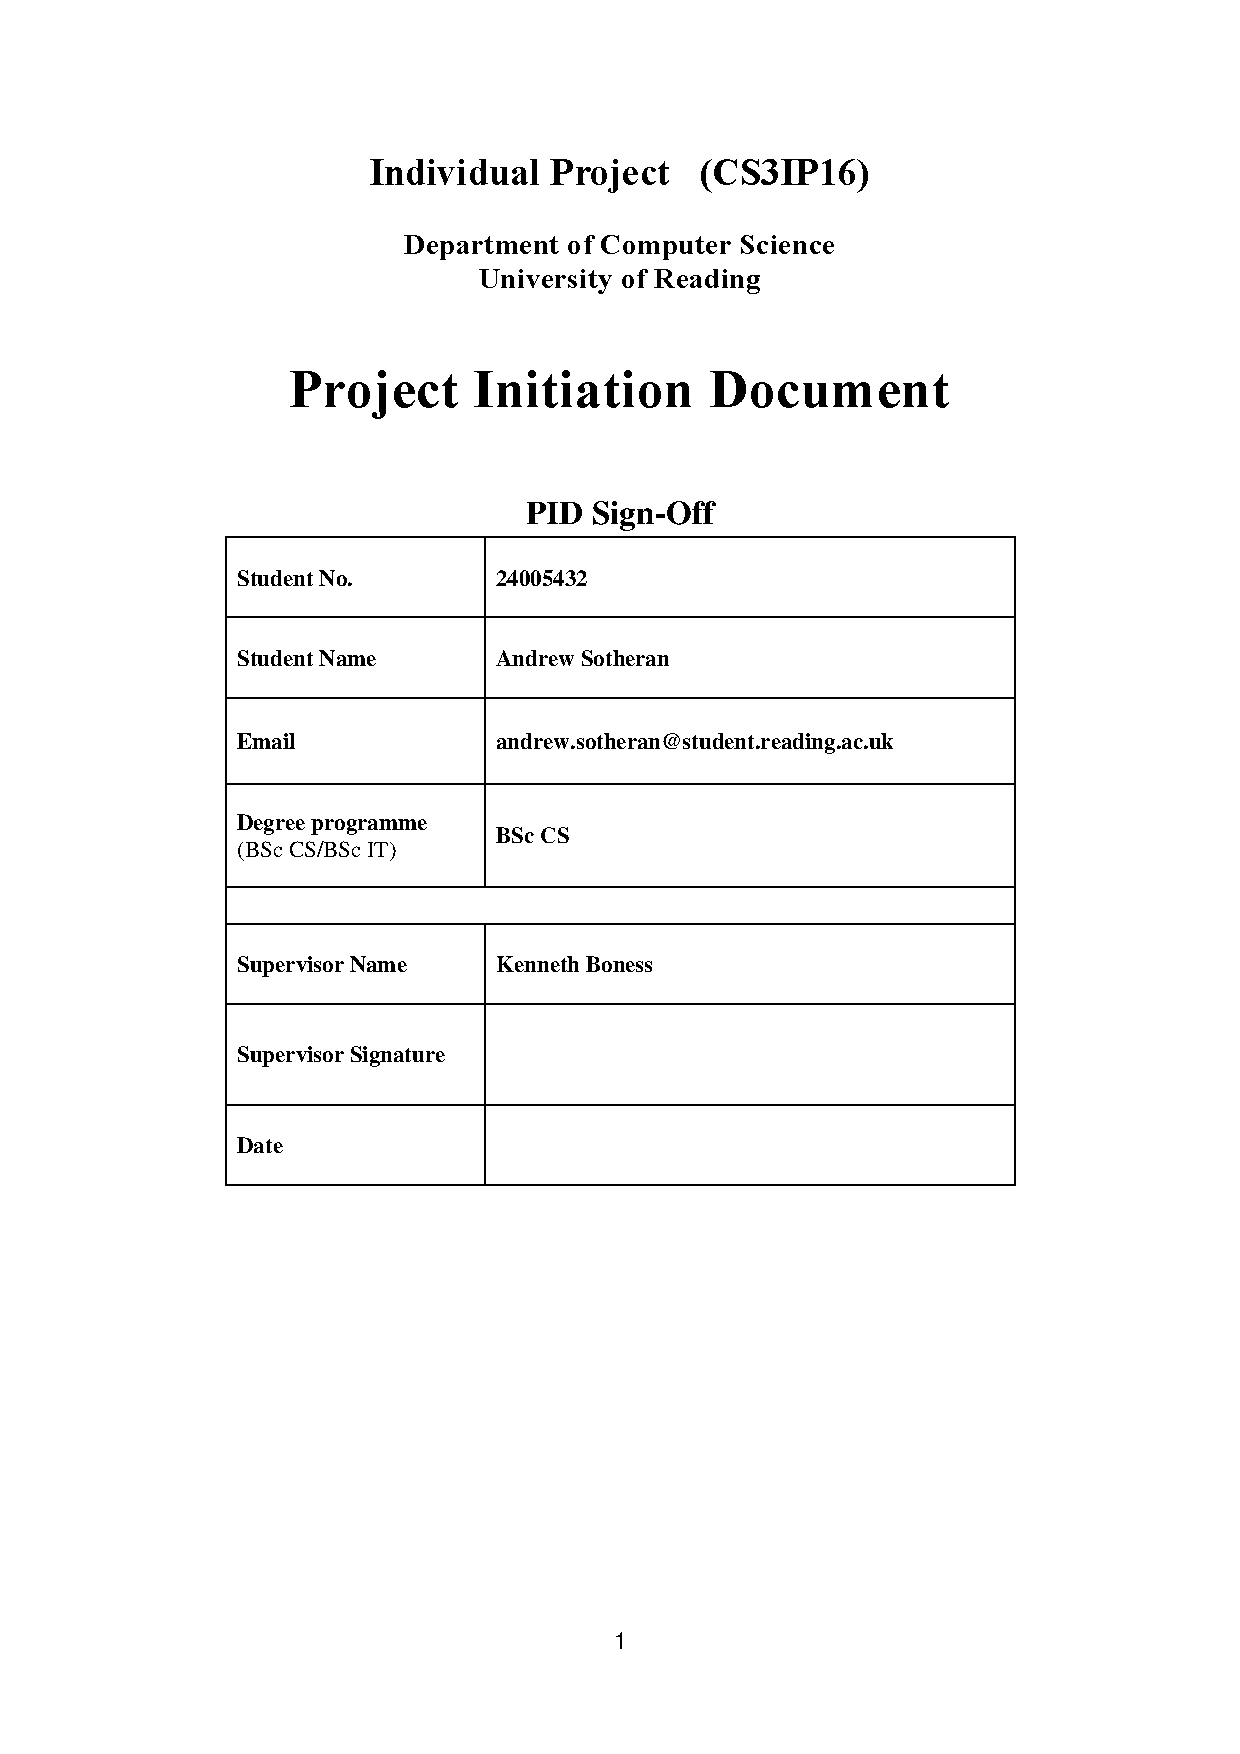
\includepdf[pages=-]{PID}
		\subsection{Appendix B - Log book}
		The log book for this project is a physical book and was handed to the School of Computer Science. Due to being a physical book, it cannot be inserted here.
	
\end{document}